
\begin{frame}{Quality of Midsurface}
\begin{itemize}[noitemsep,label=\textbullet,topsep=2pt,parsep=2pt,partopsep=2pt]
\item \textbf{Which is ``good'' Midsurface?}:
	\begin{itemize}[noitemsep,label=\textbullet,topsep=2pt,parsep=2pt,partopsep=2pt]
	\item  Mimics the original part: geometrically \& topologically. 
	\item Geometrically,  Midsurface should be in the middle. 
	\item Topologically, the connectivity between Midsurfaces should be similar to that of their corresponding sub-shapes in the parent part.
	\end{itemize}
\item \textbf{Methods of Verification}:
	\begin{itemize}[noitemsep,label=\textbullet,topsep=2pt,parsep=2pt,partopsep=2pt]
	\item Manual inspection: tedious, last resort
	\item Geometric: Not midway at connections, sampling dependent, intensive
	\end{itemize}
\end{itemize}

\end{frame}

\begin{frame}{Quality of Midsurface}
\begin{itemize}[noitemsep,label=\textbullet,topsep=2pt,parsep=2pt,partopsep=2pt]
\item Anything automatic and topological??
\item Topological (combinatorial) validation would involve, matching number of predicated topological entities with the actual ones.
\item \textbf{Advantages of Topological verification}
	\begin{itemize}[noitemsep,label=\textbullet,topsep=2pt,parsep=2pt,partopsep=2pt]
	\item  Geometry independent
	\item No sampling, just counting entities. 
	\end{itemize}
\end{itemize}

\end{frame}

\begin{frame}{Anyone tried before?}
Closest work in this regard is by Lockett\cite{Lockett2008}. 

Her objective was
\begin{itemize}[noitemsep,label=\textbullet,topsep=2pt,parsep=2pt,partopsep=2pt]
\item To evaluate the accuracy of a mid-surface model by measuring its similarity to the solid model from which it was generated. 
\item Two techniques : geometric similarity and topological similarity.
\end{itemize}
\begin{tabular}[h]{@{}p{0.48\linewidth} p{0.48\linewidth}@{}} 
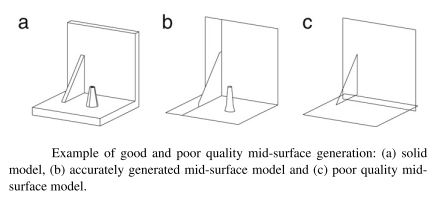
\includegraphics[width=\linewidth]{../Common/images/GoodBadMidsurf}
&
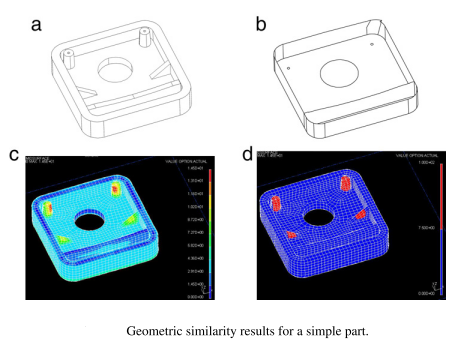
\includegraphics[width=\linewidth]{../Common/images/GeometricSimilarity}\\
\end{tabular}
\end{frame}

\begin{frame}{Lockett's Topological Similarity Assessment}
Used Angle (geometric) criteria to add edge!!!

\resizebox{0.93\linewidth}{!}{

\centering 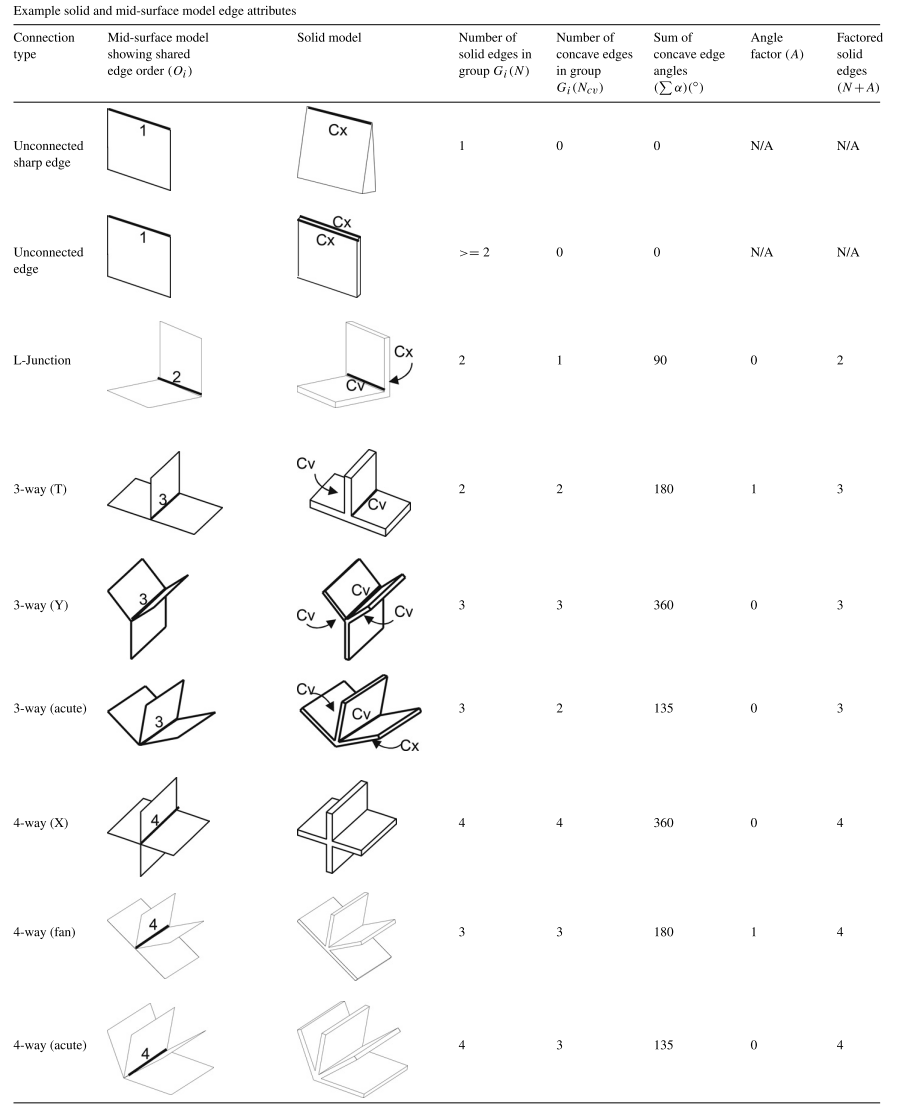
\includegraphics[width=0.015\linewidth]{../Common/images/LockettTable}

}
\end{frame}

\begin{frame}{What is Topology?}
Some geometric problems do not depend on the exact shape but the way they are put together (connected). That is Topology.  Topological equivalence:
\begin{itemize}[noitemsep,label=\textbullet,topsep=2pt,parsep=2pt,partopsep=2pt]
%[noitemsep,topsep=2pt,parsep=2pt,partopsep=2pt]
\item \textbf{Homeomorphism}: If one shape can be deformed into another without cutting or gluing. E.g. Cube, Sphere (but not torus). Letters $\mathsf{A}$ and  $\mathsf{R}$, but not  $\mathsf{B}$. Classes are ``no holes'', ``no holes with tree tails'' etc.
\begin{center}
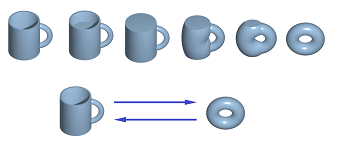
\includegraphics[width=0.2\linewidth]{../Common/images/TopologyHomeomorphism}
\end{center}

\item \textbf{Homotopy}: Equivalence if both shapes are resulted from {\em squishing} some larger object. Letters  $\mathsf{O}$ and  $\mathsf{P}$ (tail of  $\mathsf{P}$ can be squished into hole of  $\mathsf{O}$), but not  $\mathsf{B}$. Classes are larger; 'one hole', 'two holes' etc.
\end{itemize}

Many of the commercial Sheet Metal CAD modelers  represent the thin-wall shape using a geometry+topology data-structure called \textbf{Boundary Representation (Brep)}.


\end{frame}

\begin{frame}{Boundary Representation (Brep)}
Brep is composed of two parts: topology and geometry. Topological elements are, {\em shells, faces, edges, vertices} etc. They are in the descending order of the topological dimensionality.  Topological entities are:
\begin{tabular}[h]{@{}p{0.75\linewidth} p{0.2\linewidth}@{}} 

\begin{itemize}[noitemsep,label=\textbullet,topsep=2pt,parsep=2pt,partopsep=2pt]
%[noitemsep,topsep=2pt,parsep=2pt,partopsep=2pt]
\item {\em shell (s)}  is a connected set of {\em faces}
\item {\em face (f)} is a bounded portion of a {\em surface} (geometry)
\item {\em loop (l)} is a circuit of {\em edges} bounding a {\em face}
\item {\em half-edges (he)} are used to create the {\em loop}.
\item {\em edge (e)} is a bounded portion of a {\em curve} (geometry)
\item {\em vertex (v)} lies at a {\em point} (geometry). 
\end{itemize}
&
\begin{center}
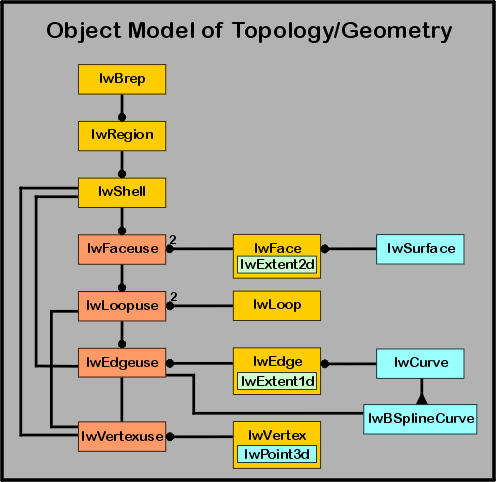
\includegraphics[width=1.2\linewidth]{../Common/images/Brep}
\end{center}

\\
\end{tabular}

Validity of the Brep model is checked using \textbf{Euler-Poincar\'e equation}.
\end{frame}

\begin{frame}{Euler-Poincar\'e Equation}
\begin{tabular}[h]{@{}p{0.7\linewidth} p{0.3\linewidth}@{}} 
Polyhedral Solids obey $v - e + f = 2$ \newline where, $v$, $e$, and $f$, are the number of vertices, edges and faces respectively.  
&
\begin{center}
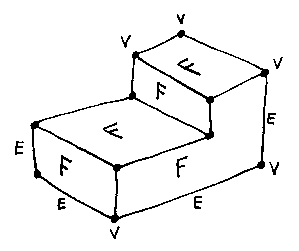
\includegraphics[width=0.65\linewidth]{../Common/images/Euler}
\end{center}
\\
\end{tabular}
More generalized form, Euler Characteristic ($\chi$)

\begin{equation}
\sum_{i=0 }^D(-1)^{i} N_{i}= \sum_{i=0}^D(-1)^{i} \beta_{i} = \chi 
\label{eqn_betti}
\end{equation}
For dimensions upto 3 ($i=3$), equation \ref{eqn_betti} reduces to
\begin{equation}
N_{0}-N_{1}+N_{2}= \beta_{0} -\beta_{1} + \beta_{2}
\label{eqn_betti3}
\end{equation}

where, $N$s are topological entities of dimension $0,1,2$ respectively and $\beta$s are Betti Numbers. $\beta_{0}$, $\beta_{1}$, $\beta_{2}$ correspond to  the number of connected components, holes and cavities, respectively \cite{Sequin}. 
\end{frame}


\begin{frame}{Manifold-Solids}
Euler-Poincar\'e equation for manifold-solids is given as 
%\vspace{-2mm}
\begin{equation}
v - e + (f - r) = 2 (s - h)
\label{eqn_manifold}
\end{equation}

Its equivalence with equation (\ref{eqn_betti3}) is as follows:

\begin{itemize}[noitemsep,label=\textbullet,topsep=2pt,parsep=2pt,partopsep=2pt]
%[noitemsep,topsep=2pt,parsep=2pt,partopsep=2pt,label={}]
\item $N_{0} = v $ : number of vertices
\item $N_{1} = e $ : number of edges
\item $N_{2} = (f - r)$ : number of faces ($f$) - additional {\em virtual-artifact} edges added corresponding to inner loops ($r$)
\item $\beta_{0} = s$ : number of components, disjoint parts ($shells$)
\item $\beta_{1} = 2h$ : number of independent closed curves drawn without splitting. Twice the genus-es $g$ or $h$. %For Torus, there are two such circles and one genus-hole. ($2h$)
\item $\beta_{2} = s$ : number of space regions created by connected surfaces. For an Open surface $\beta_{0} = 1$ but $\beta_{2}=0$. For closed surface,  $\beta_{2}$ is equal to $\beta_{0}$,  which is ($s$)
\end{itemize}

'Euler Characteristic', necessary but not a sufficient condition% for Solids.
\end{frame}

\begin{frame}{Non-manifold-Surfaces}
Solids found in the real world have the property that: on any point on the boundary, a small enough sphere at that location is split into two pieces, one inside and one outside the object. Non-manifolds do not obey this rule \cite{Krishnamurti2002}.
\begin{equation}
v - e + (f - r) = s - h
\label{eqn_nonmanifold}
\end{equation}

Its equivalence with equation (\ref{eqn_betti3}) is as follows:

\begin{itemize}[noitemsep,label=\textbullet,topsep=2pt,parsep=2pt,partopsep=2pt]
%[noitemsep,topsep=2pt,parsep=2pt,partopsep=2pt,label={}]
\item $N_{0} = v$ : number of vertices
\item $N_{1} = e$ : number of edges
\item $N_{2} = f - r $ : number of faces and inner loops ($r$)
\item $\beta_{0} = s$ : number of components, disjoint parts
\item $\beta_{1} = h$ : number of independent closed curves drawn without splitting. Inner holes are the genus-es $g$ or $h$. 
\item $\beta_{2} = 0$ : number of space regions created by connected surfaces are not present so $0$.
\end{itemize}

\end{frame}


\begin{frame}{Approaches for Topological validation}
Topological validation can be performed in two ways
\begin{itemize}[noitemsep,label=\textbullet,topsep=2pt,parsep=2pt,partopsep=2pt]
\item \textbf{Solid-to-Surface}: Find relationship between topological entities of a thin-solid and its corresponding Midsurface. See if the predicated Midsurface entities validate the non-manifold equation (Egn \ref{eqn_nonmanifold})
\item  \textbf{Surface-to-Solid}: Predict the topological entities of possible thin-wall solid that would be source of the given Midsurface.  These predicted entities can be validated against entities of the original thin-solid as well as with the manifold equation (Eqn \ref{eqn_manifold}).
\end{itemize}

\vspace{-5mm}

\begin{center}
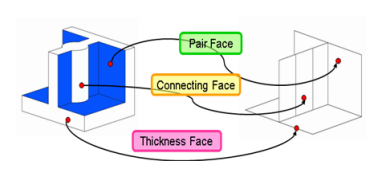
\includegraphics[width=0.6\linewidth]{../Common/images/SolidToSurface}
\end{center}

\end{frame}

\begin{frame}{Sheet Metal parts peculiarities}
Many thin-wall parts are from Sheet Metal domain. These parts are peculiar, in both, geometric as well as topological sense:
\begin{itemize}[noitemsep,label=\textbullet,topsep=2pt,parsep=2pt,partopsep=2pt]
%[noitemsep,topsep=2pt,parsep=2pt,partopsep=2pt,leftmargin=*]
\item \textbf{Constant thickness}: As Sheet Metal parts are made up of constant thickness blank.
%\item \textbf{Principal-Capping}: There are principal faces, which are part of the original blank and there are capping faces which are the side-thickness faces.
%
%%\begin{wrapfigure}{l}{0.4\linewidth}
%\begin{center} 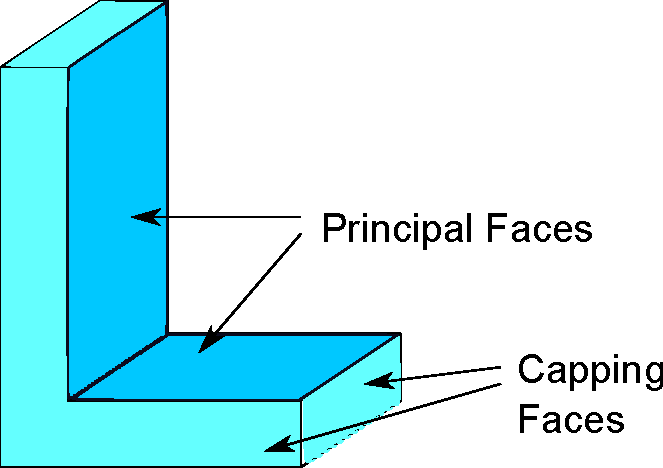
\includegraphics[width=0.34\linewidth]{../Common/images/PrincipalCappingL.pdf}
%\end{center}
%\caption{Example: Principal and Capping Faces}
%\label{fig_principalcapping}
%\end{wrapfigure} 

\item \textbf{Absences}: There are no blind holes but only through holes, if any. There are no degenerate capping-thickness faces (like 'Wedge').
%\begin{center} 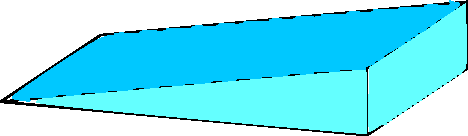
\includegraphics[width=0.34\linewidth]{../Common/images/WedgeTopology.pdf}
%\end{center}
%\item \textbf{Special Non-manifold}: Non manifoldness of their Midsurface is not in terms of edge-edge or vertex-vertex touching or partitions. Its due to its {\em surface} nature.
\item \textbf{Cavities}: There are no embedded volumes-cavities.
\end{itemize}


\begin{center}
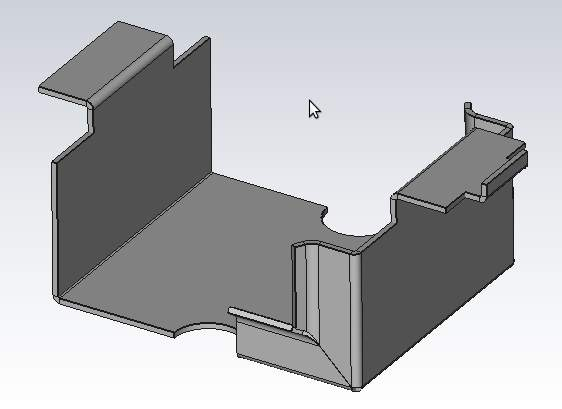
\includegraphics[width=0.45\linewidth]{../Common/images/SheetMetal}
\end{center}
\end{frame}


\begin{frame}{Usefulness of Topological Validation}
Some of the Midsurface errors can be detected using $\chi_{smm}$
\begin{itemize}[noitemsep,label=\textbullet,topsep=2pt,parsep=2pt,partopsep=2pt]
%[noitemsep,topsep=2pt,parsep=2pt,partopsep=2pt]
\item \textbf{Missing Surfaces}: Missing surface would result in less number of edges and vertices
\item \textbf{Missing Connections}: Gaps would result in less radial edges and vertices 
\end{itemize}
\begin{center}
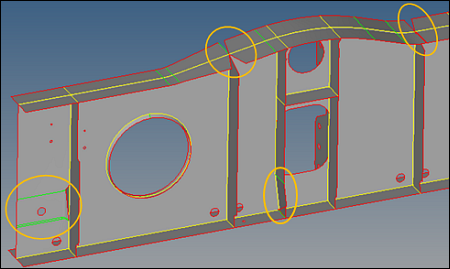
\includegraphics[width=0.5\linewidth]{../Common/images/MidsurfaceProblems}
\end{center}

\end{frame}


